\documentclass[runningheads,a4paper]{llncs}

\usepackage[latin1]{inputenc}
\usepackage{amssymb}
\usepackage{amsmath}
\setcounter{tocdepth}{3}
\usepackage{graphicx}
\usepackage{multirow}
\usepackage{rotating}
\usepackage{subfigure}
%\usepackage{subfig}
\usepackage{url}
\usepackage{caption}
\usepackage{verbatim}
%\usepackage{algorithm}
%\usepackage{algorithmic}
\usepackage{algorithm2e}

\newcommand{\keywords}[1]{\par\addvspace\baselineskip
\noindent\keywordname\enspace\ignorespaces#1}

\providecommand{\tabularnewline}{\\}

\begin{document}

\mainmatter  % start of an individual contribution

% first the title is needed
\title{Tuning Planet Wars bots for the win}

% Antonio - Un t�tulo muy 'tentativo'

% a short form should be given in case it is too long for the running head
\titlerunning{Tuning Planet Wars bots}

% the name(s) of the author(s) follow(s) next
%
% NB: Chinese authors should write their first names(s) in front of
% their surnames. This ensures that the names appear correctly in
% the running heads and the author index.
%
\author{Non A. Me%
\thanks{NoInstitute}}
%
\authorrunning{Me, N}
% (feature abused for this document to repeat the title also on left hand pages)

% the affiliations are given next; don't give your e-mail address
% unless you accept that it will be published
\institute{No Institute}

%
% NB: a more complex sample for affiliations and the mapping to the
% corresponding authors can be found in the file "llncs.dem"
% (search for the string "\mainmatter" where a contribution starts).
% "llncs.dem" accompanies the document class "llncs.cls".
%

\maketitle

%
%%%%%%%%%%%%%%%%%%%%%%%%%%%%%%%   ABSTRACT   %%%%%%%%%%%%%%%%%%%%%%%%%%%%%%%
%
\begin{abstract}
The amazing abstract
\keywords{Videogames, RTS, evolutionary algorithms, parameter tuning}
\end{abstract}

%
%%%%%%%%%%%%%%%%%%%%%%%%%%%%%%%   INTRODUCTION   %%%%%%%%%%%%%%%%%%%%%%%%%%%%%%%
%
\section{Introduction}

\begin{abstract}
\end{abstract}

\section{Evolutionary algorithms in games}
Real-Time Strategy games (RTS) are a sub-genre of strategy-based videogames in which each player controls a set of
units and structures distributed in a playing area and players take actions in real time.
In RTS games, the player is not required to wait for the results of the moves of the other players (as in turn-based games).
Well known examples of this category of games are: Command and Conquer$^{TM}$, Starcraft$^{TM}$, Warcraft$^{TM}$ and
Age of Empires$^{TM}$.

AI can be applied on RTS games in two levels~\cite{Ahlquist08Game}:
The first one, known as ``strategic'' level, is related to the behavior of a Non-Playing Character (NPC),
which is a bot that makes decisions over the whole set of units and the second level, known as ``tactical'' level,
is devoted to implementing the behavior of each one of these small units. These two levels of actions make its
study inherently difficult. This difficulty is increased by their real-time nature that most times constraints
the time that each bot can use to make a decision and also by the huge search space that is implicit in their actions.
Evolutionary algorithms have been used in videogames~\cite{Hong05Evolving,Keaveney09Evolving,Jang09Optimal}.


\section{Planet Wars}
Planet Wars\footnote{http://planetwars.aichallenge.org/} is a simple Real Time Strategy (RTS) combat-based game.
It was presented under the Google AI Challenge 2010 and has been used by several authors for the study of computational
intelligence in RTS games. Its popularity arises in the fact that it is a simplification of typical RTS games that
considers only one type of resource, one type of attack and one type of unit. \\
Planet Wars is a strategy game set in outer space. The objective is to take over all the planets on the map,
or alternatively eliminate all of your opponents ships. Figure~\ref{figplantetwars} shows a typical scenario of
a Planet Wars combat.
\begin{figure}
 \centering
 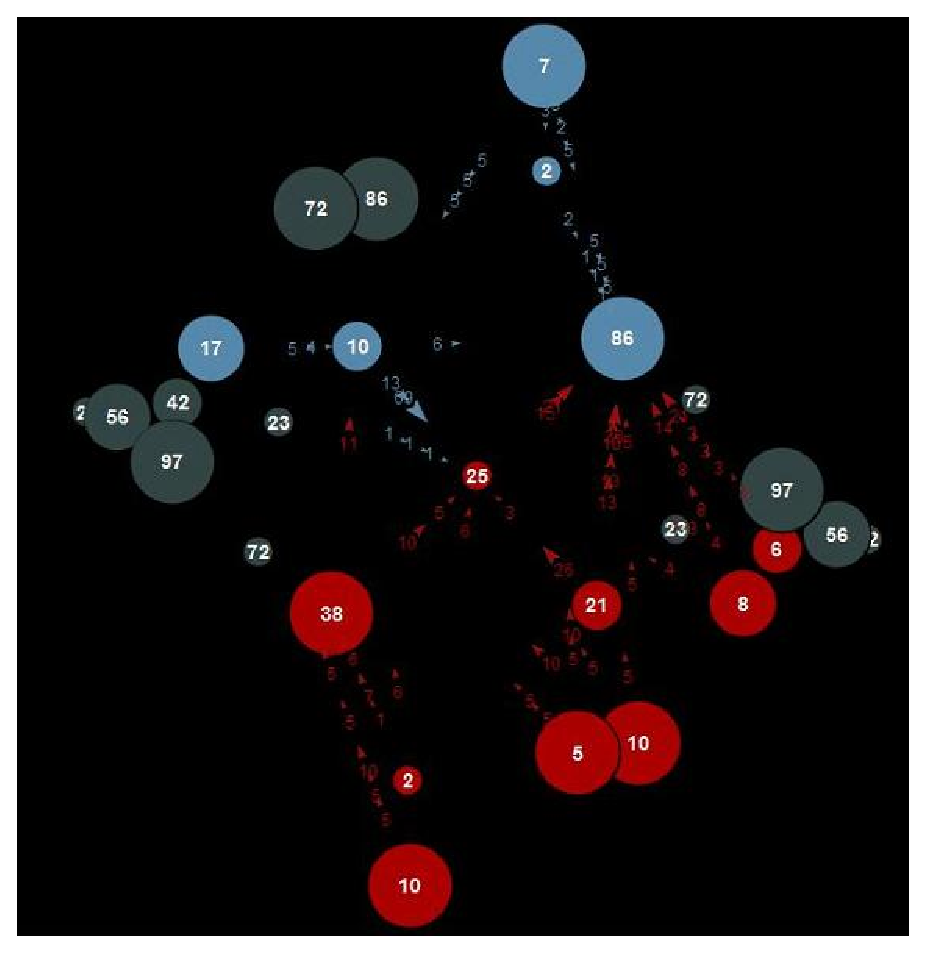
\includegraphics[scale=0.5]{images/planetwar03.eps} 
 \caption{Planet Wars scenario}\label{figplantetwars}
\end{figure}

Each bot is a function that takes a list of planets and a list of fleets and, according to this information, outputs some orders.
Each planet has the following fields/properties:
\begin{itemize}
\item Location (X and Y coordinates)
\item PlayerID of owner (For neutral planets PlayerID is zero)
\item Number of ships
\item Growth rate
\end{itemize}

The number of ships and the growth rate are both whole numbers. Each turn, the number of ships on non-neutral
planets increases according to the growth rate for that planet.\\
Fleets are the colored numbers that fly between planets. When a fleet arrives at its destination planet, one of
two things can happen:
\begin{itemize}
 \item If the destination planet is the owner of the ships arriving, they are considered as reinforcements.
 \item If the destination planet is not the owner of the ships arriving, the ships from the fleet are subtracted from
the ships that currently occupy the planet. If the number of ships is higher than the number of ships in the planet, then
the control attacking gains control of the planet. If the number of ships arriving is exactly the number of ships in the
planet, the control of the planet does not change.
\end{itemize}
A fleet has the following properties:
\begin{itemize}
\item PlayerID of owner
\item Number of ships
\item Source PlanetID
\item Destination PlanetID
\item Total trip length
\item Number of turns remaining until arrival~\footnotesize{Turn is used in this game to measure the time it takes.} 
\end{itemize}
Each player can specify as many orders as it wants during one turn. Each order specifies a source planet, a
destination planet, and a number of ships.\\
The game ends when only one player remains, or if the game has executed a maximum number of turns.

\section{Evolutionary Algorithms (EA) for optimization of autonomous agents in games}
In~\cite{Garcia-Sanchez2014Tree} Genetic Programming is used to obtain autonomous agents (bots) that play Planet Wars game.
\subsection{Representation}
Individuals are represented as binary trees formed by primitives and terminals.
\begin{itemize}
 \item Primitives correspond to ``Decisions'': logical expressions formed by a variable, a less than operator ($<$)
and a number (between $0$ and $1$). 
 \item Terminal nodes correspond to ``Actions'': each action is the name of the method to call from the planet
that executes the tree. Each method indicates to which planet send a percentage of available ships
(between $0$ and $1$).
\end{itemize}
Six variables can be considered in Decisions:
\begin{itemize}
 \item \texttt{myShipsEnemyRatio}: Ratio between the number of ships of the player and the number of ships of the enemy.
 \item \texttt{myShipsLandedFlyingRatio}: Ratio between the number of landed and flying ships of the player.
 \item \texttt{myPlanetsEnemyRatio}: Ratio between the number of planets of the player and the number of planets of the enemy.
 \item \texttt{myPlanetsTotalRatio}: Ratio between the number of planets of the player and the total number of planets (including
 neutrals and enemy planets).
 \item \texttt{actualMyShipsRatio}: Ratio between the number of ships in the specific planet that evaluates the tree and
 the total ships of the player.
 \item \texttt{actualLandedFlyingRatio}: Ratio between the number of ships landed and flying from the specific planet that
 evaluates the tree and the total ships of the player.
\end{itemize}
Twelve possible actions are considered:
\begin{itemize}
 \item \texttt{attackNearest[Enemy/Neutral]Planet}: Attack the nearest planet.
 \item \texttt{attackWeakest[Enemy/Neutral]Planet}: Attack the planet with less ships.
 \item \texttt{attackWealthiest[Enemy/Neutral]Planet}: Attack the planet with higher grown rate.
 \item \texttt{attackBeneficial[Enemy/Neutral]Planet}: Attack the more beneficial planet. The benefit of
 each planet is calculated as the ratio between its growth rate and its number of ships.
 \item \texttt{attackQuickestPlanet}: Attack the easiest planet to be conquered. The planet with lowest
 ratio between its distance (from the planet attacking) and the number of ships that its posses.
 \item \texttt{attackBase}: Attack the (neutral/enemy) planet with more ships (base).
 \item \texttt{attackRandomPlanet}.
 \item \texttt{reinforceNearestPlanet}: Reinforce the nearest own planet (from the reinforcing planet).
 \item \texttt{reinforceBase}: Reinforce the own planet with higher number of ships.
 \item \texttt{reinforceWeakestPlanet}: Reinforce the own planet with less ships.
 \item \texttt{reinforceWealthiestPlanet}: Reinforce the own planet with higher grown rate.
 \item \texttt{Do nothing}.
\end{itemize}

Figure~\ref{fig:tree} shows an example of a possible tree constructed by the algorithm. This example has a total of $7$
nodes: $3$ primitives (decisions) and $4$ terminal nodes (actions). The depth of this example is $3$ levels. 

\begin{figure}[h!]
 \centering 
 \begin{verbatim}[frame=single]
  if(randomValue<1.000)
      if(myShipsEnemyRatio<0.577)
          attackNearestEnemyPlanet(1.000);
      else
          attackNearestEnemyPlanet(0.817);
  else
      if(randomValue<0.232)
          attackBeneficiousEnemyPlanet(0.663);
      else
          attackNearestEnemyPlanet(0.916);
 \end{verbatim}
 \caption{Example of tree constructed for Planet Wars}\label{fig:tree}
\end{figure}

\subsection{Genetic Programming approach}
The genetic programming approach is shown in algorithm~\ref{alg:ea}. It corresponds to a steady state 
evolutionary algorithm that at each step generates a subset of new solutions using crossover and mutation 
operators.

\begin{algorithm}
\SetKwInOut{Input}{Input}
\SetKwInOut{Output}{Output}
\SetKwComment{Comment}{/*}{*/}
$Population \leftarrow$ \texttt{InitializePopulation}($n$) \;
$i \leftarrow 1$ \;
\Repeat{$termination\_condition$}
{\texttt{Evaluate} ($Population$) \;
$Selected \leftarrow$ \texttt{Select}($Population$) \;
$Crossed \leftarrow$ \texttt{Cross}($Selected$) \;
$Mutated \leftarrow$ \texttt{Mutate}($Crossed$) \;
$Population \leftarrow Population \cup Mutated$ \;
}
\Return;\
\caption{\texttt{$Evolutionary Algorithm$}} \label{alg:ea}
\end{algorithm}

Algorithm starts with a population of randomly generated trees. The algorithm uses a generational approach.
At each step at least half of the population (the best chosen as parents) remains in the population
and a set of new solutions are created using Sub-tree crossover and 1-node mutation.
Crossover rate has been fixed at $0.5$ and mutation rate at $0.25$.
Selection is performed using 2-tournament selection.

\subsection{Evaluation function}
The evaluation of each bot is performed considering a set of battles. Each evaluation is performed considering a set of 
opponents, a set of maps, a number of repetitions per map and a fixed number of turns. Re-evaluation is used in Genetic
approach in order to deal with the noisy nature of the fitness function. 
Fitness is calculated by:
\begin{eqnarray}
 Score_i &=& \alpha + \beta + \gamma \\
 \alpha &=& v, \alpha \in [0, NB] \\
 \beta &=& NB * \frac{t_{win} + \frac{1}{N*t_{MAX}+1}}{\frac{t_{win}}{v+1}+1}, \beta \in [0, NB*t_{MAX}] \\
 \gamma &=& \frac{t_{defeated}}{NB*t_{MAX}+1}, \gamma \in [0,1], t_{defeated} \in [0, NB*t_{MAX}]
 \label{eq:fitness}
\end{eqnarray}

where\\

\begin{tabular}{ll}
$NB$ & number of battles \\
$v$ & number of victories \\
$t_{win}$ & sum of turns used by the individual to beat opponent \\
$t_{defeated}$ & sum of turns used when the individual has been defeated \\
$t_{MAX}$ & maximum number of turns a battle lasts \\
\end{tabular}

\subsection{Crossover operator: Sub-tree crossover}
Subtree crossover~\cite{Koza94Genetic} takes two parse trees as parents and selects a subtree at
random from each parents and replace the selected subtree in one parents with the
selected subtree from the other.

\subsection{Mutation operator: 1-node mutation}
1-node mutation randomly changes the decision of a node or mutates the value with a step-size of $0.25$ 

\section{Algorithm configuration}
This section describes the approach proposed to analyze features of an evolutionary algorithm for videogames.
First, we differentiate between parameters related to the evolutionary algorithm and parameters related
to the problem.
\begin{itemize}
 \item Parameters related to the algorithm:
 \begin{itemize}
 \item Number of generations
 \item Population size
 \item Crossover operator
 \item Crossover rate
 \item Mutation operator
 \item Mutation rate
 \item Selection operator
 \item Selection size
 \end{itemize}
 \item Parameters related to the problem:
 \begin{itemize}
 \item Number of maps for evaluations
 \item Number of combats in each map
 \item Number maximum of tuns of each combat
 \end{itemize}
\end{itemize}
Considering the high computational effort required by most evolutionary algorithms for videogames we have considered to study
the effect of parameter values related to computational cost in order to determine their importance in the overall performance
of this category of evolutionary algorithms. In this study we have considered as basic cost unit: a turn of a simulation of the
game. For this, a maximum number of turns (T) will be considered as a fixed budget of each execution.\\
Then, the parameters studied are listed below:
\begin{itemize}
\item Number of generations (G)
\item Population size (P)
\item Number of maps were simulate the bot (M)
\item Number of combats in each map (n)
\item Number of maximum turns in each combat (t)
\end{itemize}

Parameter values are conditioned by:
\begin{equation}
G * P * M * n * t < T 
\end{equation}

\subsection{Tuning process}
\begin{table}
 \centering
 \begin{tabular}{ l | c | c |} 
  Parameter & Min & Max \\\hline
  Number of generations (G) & 10 & 100\\\hline
  Population size (P) & 16 & 128 \\\hline
  Number of maps (M) & 1 & 30 \\\hline
  Number of combats (n) & 1 & 5 \\
 \end{tabular}
\end{table}

Number of turns in each combat was fixed in order to tune the algorithm in fair conditions. 
Fixed budget for each run $T$ was set to $4000$.


%%%%%%%%%%%%%%%%%%%%%%%%%%%%%%%%  CONCLUSIONS  %%%%%%%%%%%%%%%%%%%%%%%%%%%%%%%%
%
\section{Conclusions}

The amazing conclusions...


%\section*{Acknowledgments}
%
%Hidden for double-blind review

\bibliographystyle{splncs03}
\bibliography{MonteroEVO2016}

\end{document}          
